

    Sentiment Analysis is the process of determining whether a piece of writing is positive, negative or neutral. A sentiment analysis system for text analysis combines natural language processing (NLP) and machine learning techniques to assign weighted sentiment scores to the entities, topics, themes and categories within a sentence or phrase.

\begin{center}
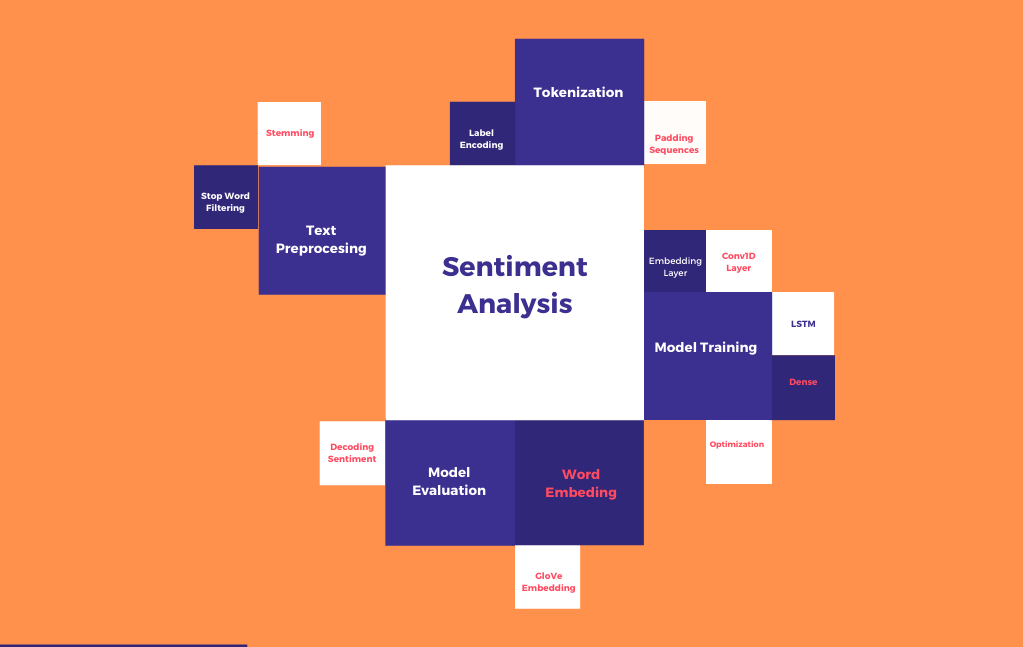
\includegraphics[scale=0.6]{sentimentanalysis.png}
\end{center}
\begin{center}
Steps of Sentiment Analysis.
\end{center}
